To safe power with a conventional receiver, it needs to be programmed in such a way, that it is kept in a sleep mode.
To check if any data was sent, it needs to wake up periodically to check for notifications.
To set this duty cycle is a trade off between response time and power consumption.
Is the period longer, the receiver is also a longer time in its sleep mode.
This period defines also directly the response time, since data can only be received in the running mode.
A wakeup receiver now allows a device to be constantly in listening mode, while consuming low energy.
Added to the system, the actual microcontroller, which coordinates the data transmission and other tasks, stays shut down with only the wakeup receiver in listening mode.
After receiving a defined pattern over this channel, the wakeup receiver generates an interrupt to wake up the microcontroller. 
It can now establish a channel over a different wireless module or execute another task.
When done, the microcontroller puts itself and all other modules except the wakeup receiver in sleep mode again.
Figure \ref{theory:wake} shows a comparison of both the conventional approach and the solution with the wakeup receiver. 
\begin{figure}[ht]
	\centering
	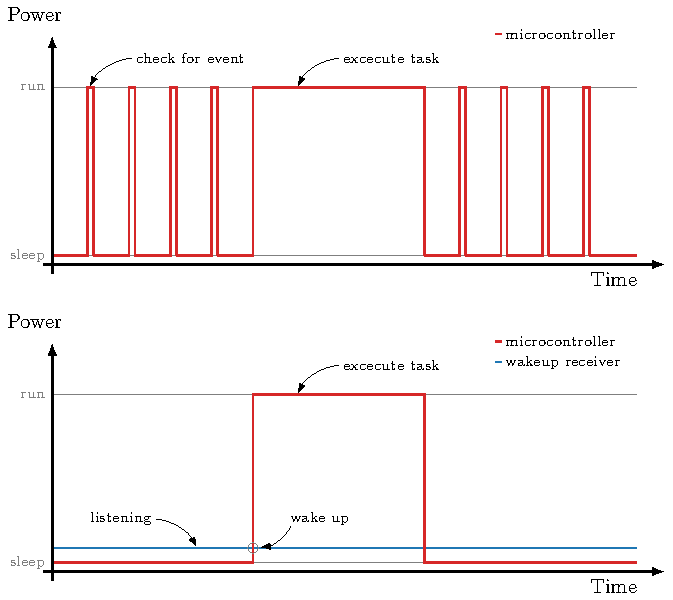
\includegraphics[width=0.9\textwidth]{2-theory/wakeup/graphics/wake_comp.pdf}
	\caption{Top: Microcontroller checks periodically for incoming data. Bottom: Constantly listening  wakeup receiver.\label{theory:wake}}
\end{figure}
One can argue that the wakeup receiver module consumes in general more power, than the microcontroller in sleep mode.
But since the microcontroller only wakes up when a task needs to be done, the overall energy consumption (area underneath the curves summarized) is going to be smaller if the occurring wakeup event comes infrequently or over longer periods of time.
The response time can be kept in the microsecond range.